\chapter{Solution approach} \label{chap:solution-apporach}

In this chapter,
we present two algorithms designed for identifying and relaxing bottlenecks in the \ac{rcpsp}.
Both algorithms aim to improve the tardiness of a selected order
by introducing relaxations to the capacity constraints in the problem instance
and finding a solution to the modified problem instance.
First, we propose an algorithm called \acf{iira}.
The \ac{iira} combines an adaptation of existing bottleneck identification approaches from the literature
with a new method for relaxing the capacity constraints.
The algorithm utilizes bottleneck identification indicators to find bottleneck resources,
selects periods with high improvement potential,
and increases the capacities of the bottleneck resources during the selected periods.
The second algorithm we propose is the \acf{ssira}.
The \ac{ssira} employs a novel approach to relaxing capacity constraints
based on finding improvement intervals in partially relaxed versions of the problem.
\ac{ssira} iteratively relaxes the capacity constraints in suffixes of an obtained schedule
and selects jobs that could start earlier following the relaxation.
The resource capacity constraints are then relaxed with respect to a small subset
of the selected jobs with improvement potential.

\todo{running example for the algorithms}

% ~~~~~~~~~~~~~~~~~~~~~~~~~~~~~~~~~~~~~~~~~~~~~~~~~~~~~~~~~~~~~~~~~~~~~~~~~~~~~~~~~~~~~~~~~~~~~~~~~~~~~~~~~~~
\section{Baseline solution} \label{sec:solution-apporach/baseline-solution}

In this section, we propose adaptations of existing bottleneck identification indicators from the literature.
Utilizing the adapted indicators, we propose the \ac{iira}
for relaxing capacity constraints of a given problem instance based on its solution.

% -----------------------------------------------------------------------------------------------------------
\subsection{Adapted identification indicators}

We adapt existing identification indicators to detect bottlenecks,
specifically the \acf{mur} and \acf{auad} indicators.
For precise definitions, see \cref{subsec:related-works/bottlenecks-in-scheduling/identification-indicators}.
        
The \ac{mur}, first utilized as a bottleneck identification indicator by \citet{Lawrence1994},
considers the ratio of executed work on a resource to the total time the resource was used.
In their study, \citet{Lawrence1994} demonstrate, that despite its simplicity,
the \ac{mur} indicator is effective at identifying long-run bottlenecks%
\footnote{
Long-run bottlenecks could be viewed as structural bottlenecks ---
see \cref{subsec:related-works/bottlenecks-in-scheduling/bottleneck-classification} for bottleneck classification.
}.


The \ac{auad}, initially proposed by \citet{Roser2001},
is more complex but remains a comprehensive indicator for identifying bottleneck resources.
For the specified resource, the sequence of all uninterrupted execution periods is computed
and the average length of those periods is considered the indicator value.
An uninterrupted period is a sequence of jobs scheduled consecutively with no idle times between them.
If there is an idle time period between two subsequent jobs,
they belong to different uninterrupted periods.

Both identification indicators consider the relationship between the total duration
of job executions on a resource and the duration for which the resource is idle.
In a Job-Shop scheduling problem,
this represents all the available information.
This concept remains applicable in the \ac{rcpsp}.
However, due to the variability of machine load over time in the \ac{rcpsp},
a binary \enquote{processing--idle} differentiation between machine states
does not provide a sufficient machine-load indication.
In the \ac{rcpsp}, we have additional information available.
By incorporating resource capacities and resource consumptions into the calculation,
we can achieve a more precise result that better corresponds to the actual machine load.
\cref{fig:MachineLoad} illustrates the difference in variability of the load between
a Job-Shop machine (\cref{fig:MachineLoad:JS})
and a \ac{rcpsp} machine (\cref{fig:MachineLoad:RCPSP}).

\begin{figure}[t]
    \centering
    
    \subfloat[Job-Shop scheduling problem]{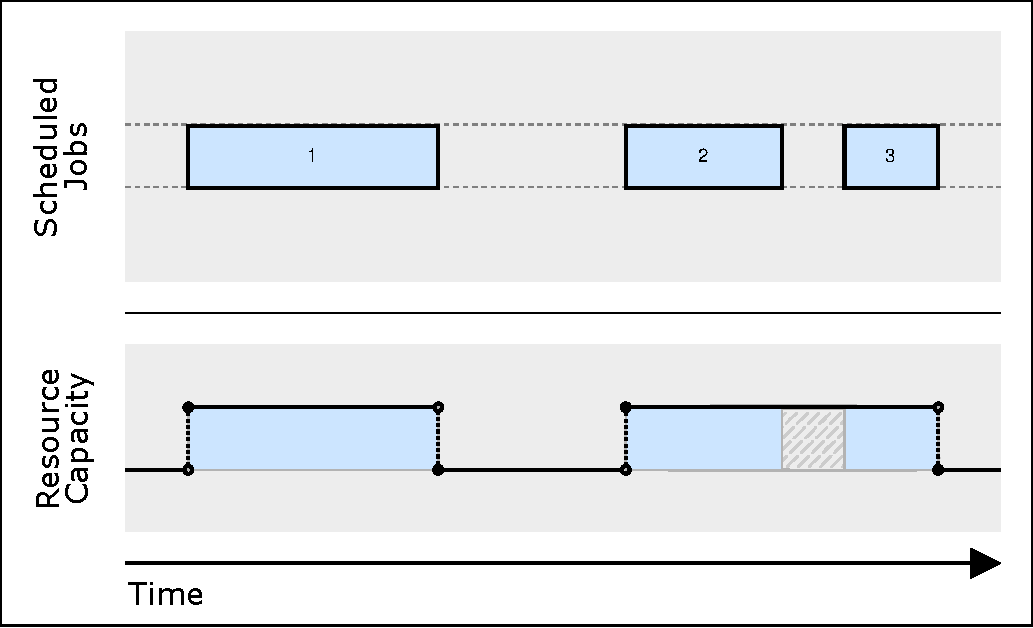
\includegraphics[width=0.7\textwidth]{img/Capacities-JobShop.pdf}\label{fig:MachineLoad:JS}}
    \\
    \subfloat[RCPSP]{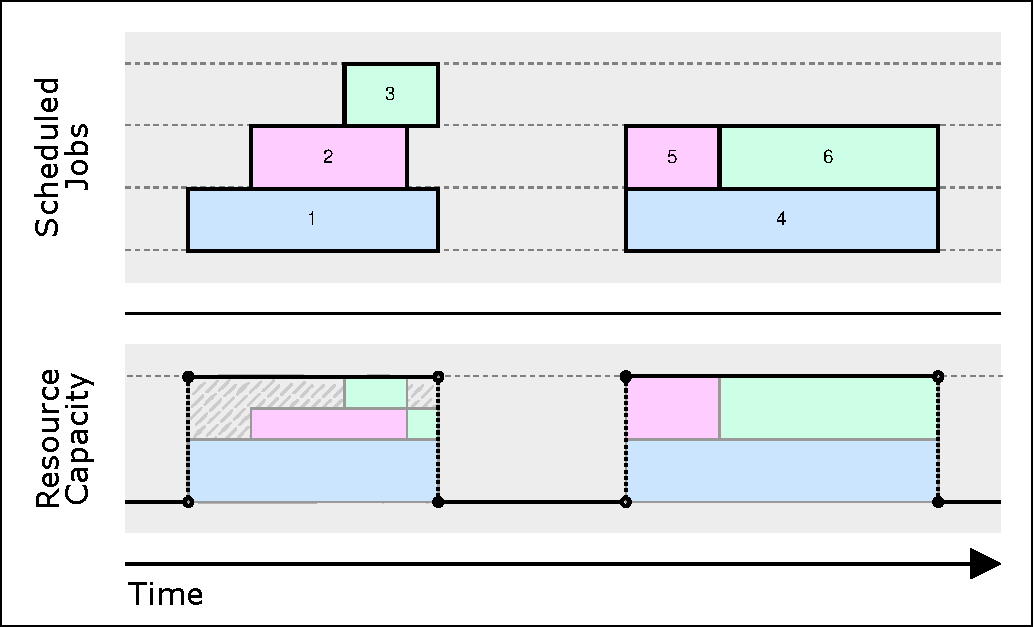
\includegraphics[width=0.7\textwidth]{img/Capacities-RCPSP.pdf}\label{fig:MachineLoad:RCPSP}}
    
    \caption{
        Examples of machine-load functions of the Job-Shop problem and the \ac{rcpsp} problem.
        The variability in the possible machine loads during job execution
        between the Job-Shop problem and the \ac{rcpsp}
        and the variability in machine loads during different periods in the \ac{rcpsp} are demonstrated.
        }
    \label{fig:MachineLoad}
\end{figure}

We propose \acf{mrur} as the adaptation of \ac{mur} and \acf{auau} as the adaptation of \ac{auad}.
For a resource $k$, the \ac{mrur} is defined as:
$$
\indMRUR{k} \defeq \frac{\sum_{j \in \Jobs} (\duration{j} \cdot \consumption{j}{k})}%
                        {\sum_{t=1}^{C_{\max}} \capacity{k}{t}},
$$
where $C_{\max} \defeq \max_{j \in \Jobs} \jobend{j}$%
\footnote{In the scheduling literature,
$C_{\max}$ is referred to as the \emph{makespan} of the project.
Minimizing project makespan is a common optimization goal in scheduling,
and it is a simpler alternative to the total weighted tardiness we use.}.
For a resource $k$, the \ac{auau} is defined as:
$$
\indAUAU{k} \defeq \frac{\sum_{i=1}^{A_k} \indPRU{k}{i}}%
                        {A_k},
$$
where the \acf{pru} of resource $k$ during the uninterrupted active period $i$
is defined as
$$
\indPRU{k}{i} \defeq \frac{\sum_{j \in \JobsOnResourceInPeriod{k}{i}}
                                \duration{j} \cdot \consumption{j}{k}}%
                          {\sum_{t=a_{ki}^{S}}^{a_{ki}^{E}} \capacity{k}{t} }.
$$
For a resource $k$,
$(a_{k1}^{S}, a_{k1}^{E}), \dots, (a_{kA_k}^{S}, a_{kA_k}^{E})$
is the the sequence of \emph{uninterrupted active periods},
where $a_{ki}^{S} \in \intinterval{1}{\horizon}$ denotes the start of the period $i$
and $a_{ki}^{E} \in \intinterval{1}{\horizon}$ denotes the end of the period $i$.
Similar to the definition of \ac{auad} but with differences induced by non-unit capacities,
an uninterrupted active period is a maximal set (maximal in terms of inclusion)
of jobs scheduled consecutively or in parallel with no idle time
occurring on the considered resource during the period.
Two jobs are in the same uninterrupted active period, if and only if
the execution intervals of the jobs overlap
or the considered resource is not idle between the execution intervals of the jobs.
The sequence of uninterrupted active periods of a resource is the transitive closure of this relation
on jobs executed on the resource.
Here, as opposed to the \ac{auad},
we do not consider the duration of the periods,
but the individual jobs executed during each of the periods,
specifically their durations and consumptions of the evaluated resource.

In the formula for $\indPRU{k}{i}$,
$\JobsOnResourceInPeriod{k}{i} \defeq \{ j \in \JobsOnResource{k} : a_{ki}^{S} \leq \jobstart{j} \leq a_{ki}^{E} \}$
is the set of jobs executed on resource $k$ during the uninterrupted active period $i$.
Recall from \cref{subsec:related-works/bottlenecks-in-scheduling/identification-indicators} that
$\JobsOnResource{k} = \{ j \in \Jobs : \consumption{j}{k} > 0 \}$.

Having proposed bottleneck identification indicators for our \ac{rcpsp} variant,
we will formulate an algorithm utilizing those indicators in the following section.

% -----------------------------------------------------------------------------------------------------------
\subsection{Identification Indicator-based Relaxing Algorithm} \label{subsec:solution-approach/baseline-solution/iira}

In this section, we formulate the \acf{iira}.
\ac{iira} employs a specified bottleneck identification indicator to identify bottleneck resources.
It calculates the granular resource load function
and uses its convolution with a suitably chosen kernel function
to determine the improvement potential for granular periods.
Finally, it relaxes capacity constraints in granular periods with the greatest improvement potential.
Following this, a solution is obtained for the relaxed problem instance,
and the proposed capacity relaxations are reduced to only include those utilized by the new solution.
The \acf{iira} is given in \cref{alg:identification-indicator-relaxing-algorithm}.

\begin{algorithm}[t]
\caption{\acf{iira}}
\label{alg:identification-indicator-relaxing-algorithm}
\begin{algorithmic}[1]

\Params  Identification indicator $\algIndicator$, granularity $\algGranularity$, convolution mask $\algConvolution$,
\Paramsc iterations limit $\algMaxiter$, improvement periods limit $\algMaxperiods$,
\Paramsc capacity improvement $\algImprovement$
\Input  Solution $\Schedule$ to a problem instance $\Instance$

\State $PC \gets \lceil \horizon / \algGranularity \rceil$
       \Comment The number of granular periods
\State $\Instance^* \gets \Instance$, $\Schedule^* \gets \Schedule$
       \Comment Modified instance and its solution, initially
       \Statecr copies of the original instance and solution
\Repeat \label{alg:iira/repeat}
    \State Evaluate $\Schedule^*$ using $\algIndicator$, obtaining:
           $\algIndicator_k \;\forall k \in \Resources$ \label{alg:iira/evaluation}
    \State Identify bottleneck resource:
           $k^* \gets \argmax_k \algIndicator_k$ \label{alg:iira/identification}
    \State Compute granular resource load for $k^*$: \label{alg:iira/granular-load}
    \Statec{3} $\resourceLoad{k^*} \gets $ \Callref{GranularResourceLoad}%
                                                   {$k^*$, $\Instance^*$, $\Schedule^*$, $PC$}%
                                                   {alg:granular-resource-load}
    \State Compute improvement potential of periods: $\Psi \gets \resourceLoad{k^*} * \algConvolution$ \label{alg:iira/convolution}
    \State Find improvement periods: \label{alg:iira/periods}
    \Statec{3} $p_1, \dots, p_{\algMaxperiods} \gets$
            periods with the highest potential $\Psi(i)$
    \For {$i \in \{p_1, \dots, p_{\algMaxperiods}\}$}
        \State $\capacityf{k^*}^* \gets$ \Callref{IncreaseGranularPeriodCapacity}%
                                                 {$i$, $\capacityf{k^*}^*$, $\algGranularity$, $\algImprovement$}%
                                                 {alg:increase-granular-period-capacity} \label{alg:iira/capacity-increase}
    \EndFor
    \State Find solution $\Schedule^*$ to the modified instance $\Instance^*$ \label{alg:iira/modified-solution}
    \State $\capacityf{1}^*, \dots, \capacityf{m}^* \gets$ \Callref{ReduceCapacityChanges}%
                                                                   {$\Instance^*$, $\Schedule^*$, $\capacityf{1},$ \dots, $\capacityf{m}$}%
                                                                   {alg:reduce-capacity-changes} \label{alg:iira/reduction}
    \State $\Additions^{\Instance^*}, \Migrations^{\Instance^*} \gets $
           \Callref{FindAdditionsAndMigrations}%
                   {$\Instance^*$, $\Schedule^*$}%
                   {alg:find-additions-and-migrations} \label{alg:iira/additions-migrations}
\ForIter{$\algMaxiter$} \label{alg:iira/for-iters}

\Output  Modified instance $\Instance^*$ and its solution $\Schedule^*$,
\Outputc additions $\Additions^{\Instance^*}$, migrations $\Migrations^{\Instance^*}$
\Statex
\Note In the call to \Call{ReduceCapacityChanges}{} (statement 12),
      $\capacityf{k^*}$ from the~original instance is given as the original capacity function of the resource $k^*$.

\end{algorithmic}
\end{algorithm}

The algorithm consists of a main loop (lines~\ref{alg:iira/repeat}--\ref{alg:iira/for-iters}),
the input of which is a problem instance and its solution,
the output of which is a modified problem instance and its solution.
We describe the individual steps performed by the algorithm in the following outline.

\begin{steps}
    \item
    First, the solution is evaluated using the given identification indicator
    and the bottleneck resource is identified by its maximal value of the identification indicator
    (lines~\ref{alg:iira/evaluation} and~\ref{alg:iira/identification}).

    \item
    The granular load of the bottleneck resource is computed
    and the improvement potentials for granular periods are computed
    using convolution (lines~\ref{alg:iira/granular-load} and~\ref{alg:iira/convolution}).
    The granular load of a resource indicates how the resource is being utilized during granular periods.
    High utilization could indicate a potential bottleneck.
    However, it is uncertain whether the bottleneck occurs in the highly-utilized granular period,
    or whether the high utilization is a consequence of a bottleneck
    in a preceding or following granular period.
    This is why the granular load is convolved with a kernel function of choice,
    which propagates the information about high resource utilization
    to consecutive granular periods.
    The result of the convolution is trimmed to only contain "valid" values,
    i.e. values computed directly on the interval $\intinterval{1}{PC}$.
    \label{alg/iira-steps/identification}

    \item
    A small subset of granular periods is selected for the increase in capacity.
    The granular periods with the highest improvement potentials are chosen (line~\ref{alg:iira/periods}).
    The capacity of the bottleneck resource is increased during the selected granular periods
    by a specified amount (line~\ref{alg:iira/capacity-increase}).
    The modified resource capacity function of the bottleneck resources forms,
    together with the unchanged capacity functions of other resources,
    a new modified problem instance.
    Note that the algorithm does not consider the target order~$\targetOrder$ in any way
    when identifying bottlenecks (\cref{alg/iira-steps/identification})
    nor when selecting granular periods for capacity constraints relaxation.

    \item
    Finally, a new solution to the modified problem instance is found (line~\ref{alg:iira/modified-solution}).
    Based on this solution,
    reduced capacity functions are computed to exclude capacity relaxations
    not utilized in the solution (line~\ref{alg:iira/reduction}).
    The reduction involves the capacity functions of all the resources, not only of the bottleneck resource.
    This is because, in subsequent iterations of the algorithm,
    the introduction of new relaxations often leads to changes in the solution schedule.
    Such changes might cause previous relaxations to no longer be necessary,
    so in turn, every resource capacity function is reduced.
    Note that the function \algnameref{ReduceCapacityChanges}{alg:reduce-capacity-changes}
    takes the original resource capacity functions as input
    and the reductions are made with respect to them.
    As a final step, capacity migrations are computed in the reduced capacity functions
    to best utilize the existing unused capacities (line~\ref{alg:iira/additions-migrations}).
    Any remaining capacity requirements are then fulfilled with capacity additions.
\end{steps}

The algorithm utilizes multiple additional procedures and functions.
For brevity, we exclude the detailed specifics of the procedures
and instead offer short overviews of each procedure.
Complete pseudocodes of the procedures are available in \cref{sec:attachments/algorithms-functions-procedures}.

\begin{itemize}
    \item \algnameref{GranularResourceLoad}{alg:granular-resource-load}
        computes a granular resource load for a given resource.
        The granular load is a function mapping granular periods to the cumulative sum of the load
        of the resource over the specified granular period.
        Example of a computed granular load can is illustrated in \cref{fig:granular-load}.

        \begin{figure}
            \centering
            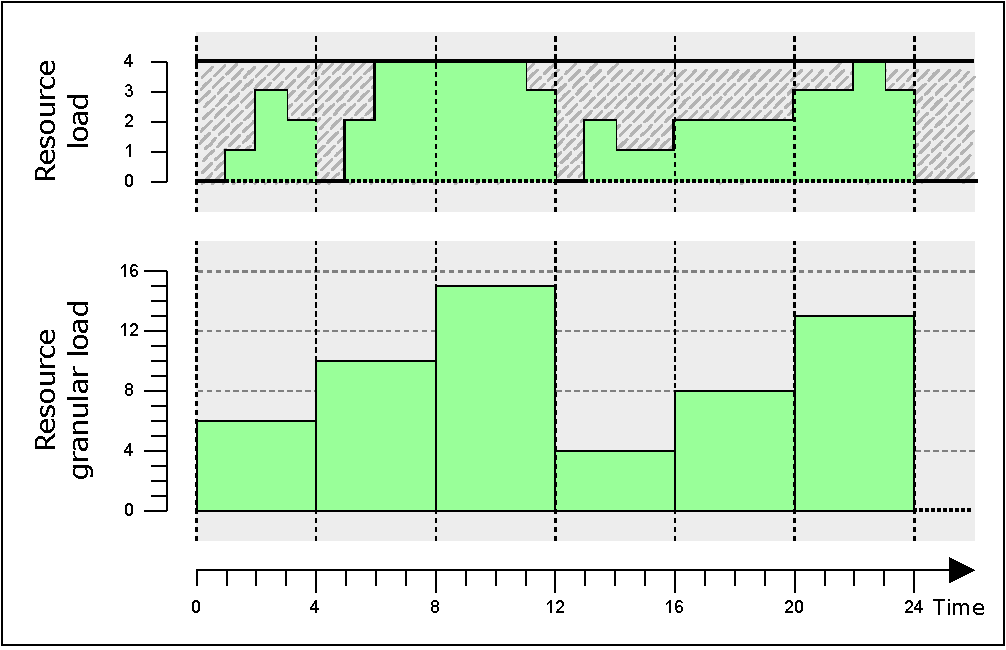
\includegraphics[width=\textwidth]{img/GranularLoad.pdf}
            \caption{
                Resource granular load example.
                The first panel illustrates the resource load representing the consumption of jobs.
                The second panel illustrates the computed granular load with the granularity of 4 time periods.
                }
            \label{fig:granular-load}
        \end{figure}
        
    \item \algnameref{IncreaseGranularPeriodCapacity}{alg:increase-granular-period-capacity}
        increases the values of the given capacity function during the specified granular period.
        The capacity is increased in each time period covered by the granular period,
        determined by the specified granularity.

    \item \algnameref{ReduceCapacityChanges}{alg:reduce-capacity-changes}
        constructs reduced capacity functions for the given problem instance based on the original resource functions
        and the actual load of the instance resources (computed from the given solution).
        This function reduces redundant capacity additions introduced by former relaxations
        so that the resource capacity functions do not contain capacity additions not utilized by the solution.

    \item \algnameref{FindAdditionsAndMigrations}{alg:find-additions-and-migrations}
        finds capacity additions and migrations,
        as defined in \cref{subsec:problem-statement/bottlenecks/resource-capacity-modifications},
        for the resources of the given problem instance.
        In the same section,
        we discussed that in real-world production systems
        capacity migrations are preferred over capacity additions due to their comparatively small execution cost.
        Thus, we first find all possible migrations to utilize existing capacities.
        Then, when no other migrations are possible, the remaining capacity requirements are fulfilled
        by introducing capacity additions.
\end{itemize}

\todo{REVISION of algorithms}

% ~~~~~~~~~~~~~~~~~~~~~~~~~~~~~~~~~~~~~~~~~~~~~~~~~~~~~~~~~~~~~~~~~~~~~~~~~~~~~~~~~~~~~~~~~~~~~~~~~~~~~~~~~~~
\section{Extended solution} \label{sec:solution-apporach/extended-solution}

In this section, we present a novel method for detecting bottlenecks
and relaxing related constraints in the \ac{rcpsp}.
The method is based on finding improvement intervals
in partially relaxed versions of the given problem.
A small subset of the improvement intervals is then selected and capacity constraints
corresponding to the selected improvement intervals are relaxed.
The primary goal is to identify relaxations that focus specifically on the target order.
By doing so, we hope to achieve great improvements in the tardiness of the target order
while maintaining low capacity modification costs and induced schedule differences.
In doing so, we aim to improve the tardiness of the target order
while keeping capacity modification costs and the induced schedule differences to a minimum.

% -----------------------------------------------------------------------------------------------------------
\subsection{Preliminaries} \label{subsec:solution-approach/extended-solutin/preliminaries}

Before we formulate the \acl{ssira},
we need to state a few definitions and ideas upon which the algorithm is designed.
First, we define the \emph{suffix-relaxed schedule} as a modification of an obtained schedule solution
where the algorithm finds improvement intervals.
We then define the \emph{left-shift closure} as a tool
for focusing the search for improvement intervals towards improving the tardiness of the target order.

\begin{defn}[Suffix-relaxed schedule] \label{def:suffix-relaxed-schedule}
    Let $\Schedule = (\jobstart{1}, \dots, \jobstart{n})$ be a schedule to a problem instance $\Instance$.
    Given a time period $t \in \intinterval{1}{\horizon}$,
    the \emph{suffix-relaxed schedule} for the time period $t$ is given by
    $\relaxedSchedule{t} = (\relaxedjobstart{t}{1}, \dots, \relaxedjobstart{t}{n})$, where
    $$
    \relaxedjobstart{t}{j} \defeq \begin{cases}
        \jobstart{j} & \text{if $\jobstart{j} \leq t$;} \\
        \max\left\{\relaxedjobstart{t}{j} : \precedence{i}{j} \in \Precedences \right\} & \text{otherwise.}
    \end{cases}
    $$
\end{defn}

\begin{figure}
    \centering
    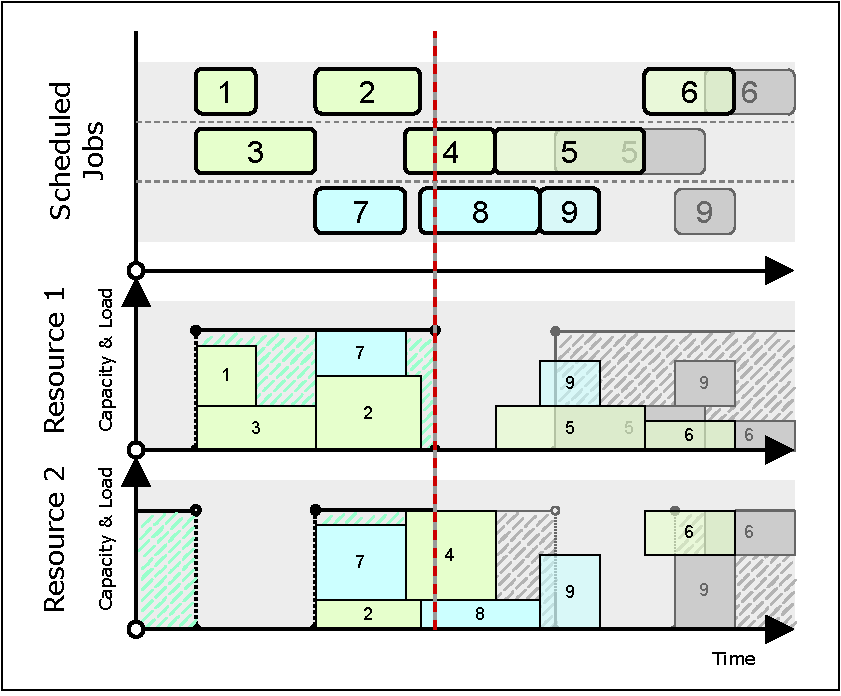
\includegraphics[width=\textwidth]{img/Schedule-Relaxed.pdf}
    \caption{
        Example of a suffix-relaxed schedule based on the schedule given in \cref{fig:schedule}.
        The red vertical line represents the time period for which the suffix-relaxed schedule was computed.
        The resource capacity constraints were relaxed for jobs 5, 6, and 9
        as they were scheduled later than the specified time period.
        In the suffix-relaxed schedule,
        the start times of those jobs are constrained only by precedence constraints.
        We observe that in the relaxed schedule,
        job 9 would require only small capacity additions on both resources,
        should it be scheduled on them.
        Moreover, most of the requirements could be satisfied
        by migrating unused capacities between the resources.
        }
    \label{fig:schedule-relaxed}
\end{figure}

For a given job $j$, the value of $\relaxedjobstart{t}{j}$
depends only on the values $\relaxedjobstart{t}{i}$ of its precedence predecessors $i$,
given by precedences $\precedence{i}{j}$.
Since the precedence graph is directed and acyclic,
all values of $\relaxedSchedule{t}$ are well-defined and the definition is correct.

The suffix-relaxed schedule for a time period $t$ is a modification of the original schedule
where the start times of jobs starting in time periods up to $t$ remain unchanged,
and the start times of jobs scheduled to start later can be shifted to earlier time periods,
constrained only by precedence constraints.
This essentially relaxes resource capacity constraints for all jobs that, in the original schedule,
start after the time period $t$.

The idea is that a job scheduled during the later time periods could not be scheduled earlier
due to the lack of remaining capacity on the required resources,
assuming sufficient slack in precedence constraints.
By fully relaxing the resource capacity constraints in the suffix of a schedule,
we can compute potential starting times for jobs scheduled in that suffix,
had they not been constrained by the resource capacity constraints.
Following this, we can observe the potential improvements in the starting times
and the consequent required resource capacity relaxations.

\begin{defn}[Left-shift closure] \label{def:left-shift-closure}
    Let $\Schedule = (\jobstart{1}, \dots, \jobstart{n})$ be a schedule to a problem instance $\Instance$.
    A \emph{left-shift closure} of a job $j \in \Jobs$ is the set $\closure{j}~\subseteq~\Jobs$, where:
    \begin{conditions}
        \item
            $j \in \closure{j}$ \label{def:closure/base}

        \item
            All precedence predecessors directly preceding in the schedule are included.
            $$
            (\forall \precedence{i}{j} \in \Precedences):
            \jobend{i} = \jobstart{j} \implies \closure{i} \subset \closure{j}
            $$ \label{def:closure/precedence}
            \vspace{-2em}

        \item
            All jobs consuming a common resource directly preceding in the schedule are included.
            $$
            (\forall k \in \Resources, \consumption{j}{k} > 0)
            (\forall i \in \JobsOnResource{k}):
            \jobend{i} = \jobstart{j} \implies \closure{i} \subset \closure{j}
            $$ \label{def:closure/resource-precedence}
            \vspace{-2em}

        \item
            If $j$ is scheduled exactly at the start of a working shift,
            all jobs scheduled at the end of the previous working shift are included.
            \begin{multline*}
            (\forall k \in \Resources, \consumption{j}{k} > 0, \capacity{k}{\jobstart{j}-1} = 0)
            (\forall i \in \JobsOnResource{k}):
            \\
            \mathrm{ps}_k(\jobstart{j}) - \duration{j} \leq \jobend{i} \leq \mathrm{ps}_k(\jobstart{j})
            \implies \closure{i} \subset \closure{j}
            \end{multline*} \label{def:closure/shift-pause-precedence}
            where $\mathrm{ps}_k(t) \defeq \max\{t^\prime \in \intinterval{1}{t-1} : \capacity{k}{t^\prime} > 0\}$.
    \end{conditions}
\end{defn}

\begin{figure}[t]
    \centering
    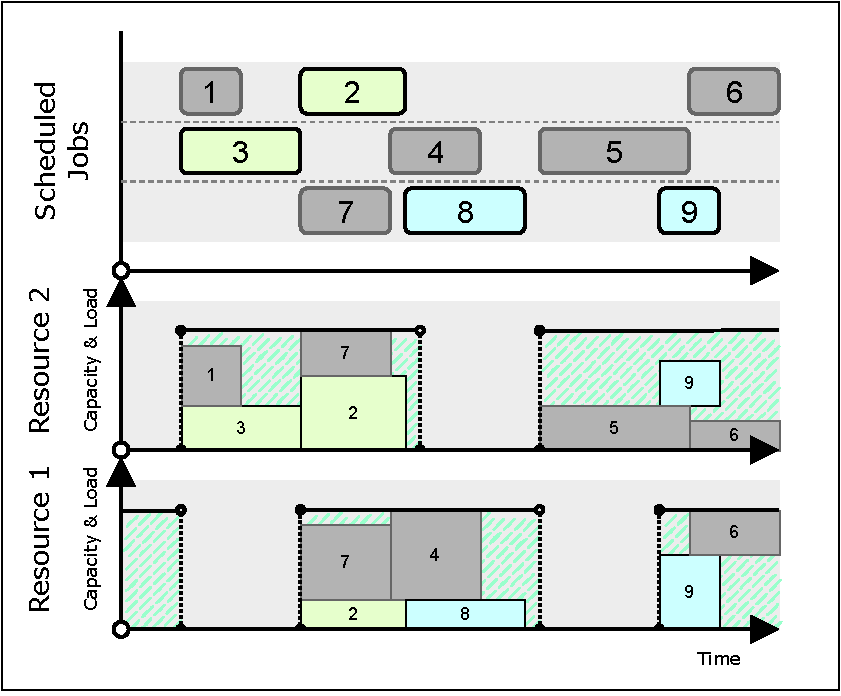
\includegraphics[width=\textwidth]{img/Schedule-Closure.pdf}
    \caption{
        Example of a left-shift closure computed for the job 9 in the schedule given in \cref{fig:schedule}.
        Here, the left-shift closure of the job 9 is the set $\closure{9} = \{ 3, 7, 8, 9 \}$.
        The included jobs are highlighted; jobs not included are dimmed.
        Job 9 is trivially included by \cref{def:closure/base}.
        Job 8 is included by \cref{def:closure/shift-pause-precedence} --- pauses in resource working shifts.
        Job 7 is included by \cref{def:closure/precedence} --- precedence predecessor of the job 8.
        Job 3 is included by \cref{def:closure/resource-precedence} --- resource predecessor of the job 7 on resource 1.
        }
    \label{fig:schedule-closure}
\end{figure}

The left-shift closure of a job $j$ defines the set of all jobs
preventing the job $j$ from starting in an earlier time period.
The only exception to this interpretation is the \cref{def:closure/base},
which simplifies the inductive definition.

\Cref{def:closure/precedence} states that a direct predecessor $i$ of the job $j$,
indicated by the precedence constraint $\precedence{i}{j}$,
is included in $\closure{j}$ if the jobs are scheduled consecutively.
Jobs $i$ and $j$ are scheduled consecutively if the execution of the job~$i$ ends
at the exact same time period where the execution of the job $j$ starts,
i.e. $\jobend{i} = \jobstart{j}$.

\Cref{def:closure/resource-precedence} involves all jobs scheduled consecutively with the job $j$,
which share at least one required resource.
Jobs can be executed on multiple resources,
but sharing just one resource is sufficient for the jobs to influence each other.
This resource requirement overlap can delay the job $j$ if its predecessor job $i$'s resource consumption
prevents the job $j$ from being scheduled earlier.

Lastly, \cref{def:closure/shift-pause-precedence} involves jobs at the end of previous working shifts.
Assuming sufficient slack in precedence constraints,
the job $j$ starts exactly at the start of a working shift because
it could not have been scheduled at the end of the previous working shift
due to the lack of remaining capacities on its required resources.
Jobs scheduled at the end of the previous working shift consume the required resources
and thus prevent the job $j$ from being scheduled there.

% -----------------------------------------------------------------------------------------------------------
\subsection{Schedule Suffix Interval Relaxing Algorithm} \label{subsec:extended-solution/schedule-suffix-interal-relaxing-algorithm}

Having presented the main concepts in the previous section,
we now formulate the \acf{ssira} in \cref{alg:schedule-suffix-interval-relaxing-algorithm}.
The formulation of the algorithm itself is quite simple.
The core procedure is encapsulated in the
\algnameref{Find\-Intervals\-To\-Relax}{alg:find-intervals-to-relax} function,
formulated in \cref{alg:find-intervals-to-relax}.


\begin{algorithm}[t]
\caption{\acf{ssira}}
\label{alg:schedule-suffix-interval-relaxing-algorithm}
\begin{algorithmic}[1]

\Params  Iterations limit $\algMaxiter$, improvement intervals limit $\algMaxintervals$,
\Paramsc interval sort key $\algSortkey$
\Input  Solution $\Schedule$ to a problem instance $\Instance$, target order $\targetOrder$

\State $\Instance^* \gets \Instance$, $\Schedule^* \gets \Schedule$
       \Comment Modified instance and its solution, initially
       \Statecr copies of the original instance and solution
\Repeat \label{alg:ssira/repeat}
    \State $\chi_1, \dots, \chi_{\algMaxintervals} \gets$ \Callref{FindIntervalsToRelax}%
                                                                  {$\Instance^*$, $\Schedule^*$, $\algMaxintervals$, $\algSortkey$, $\targetOrder$}%
                                                                  {alg:find-intervals-to-relax}
                                                                  \label{alg:ssira/ints}
    \State $\capacityf{1}^*, \dots, \capacityf{m}^* \gets$ \Callref{ModifyResourceCapacities}%
                                                                   {$\Instance^*$, $\chi_1, \dots, \chi_{\algMaxintervals}$}%
                                                                   {alg:modify-resource-capacities}
                                                                   \label{alg:ssira/modify}
    \State Find solution $\Schedule^*$ to the modified instance $\Instance^*$ \label{alg:ssira/solution}
    \State $\capacityf{1}^*, \dots, \capacityf{m}^* \gets$ \Callref{ReduceCapacityChanges}%
                                                                   {$\Instance^*$, $\Schedule^*$, $\capacityf{1},$ \dots, $\capacityf{m}$}%
                                                                   {alg:reduce-capacity-changes}
                                                                   \label{alg:ssira/reduction}
    \State $\Additions^{\Instance^*}, \Migrations^{\Instance^*} \gets $
           \Callref{FindAdditionsAndMigrations}%
                   {$\Instance^*$, $\Schedule^*$}%
                   {alg:find-additions-and-migrations}
                   \label{alg:ssira/additions-migrations}
\ForIter{$\algMaxiter$} \label{alg:ssira/for-iters}

\Output  Modified instance $\Instance^*$ and its solution $\Schedule^*$,
\Outputc additions $\Additions^{\Instance^*}$, migrations $\Migrations^{\Instance^*}$
\end{algorithmic}
\end{algorithm}


\begin{algorithm}[t]
\caption{FindIntervalsToRelax}
\label{alg:find-intervals-to-relax}
\begin{algorithmic}[1]

\Input  Problem instance $\Instance$, its solution $\Schedule$, improvement intervals limit $\algMaxintervals$,
\Inputc interval sort key $\algSortkey$, target order $\targetOrder$

\For {$t \in \intinterval{1}{\horizon}$}
    $\relaxedSchedule{t} \gets$ \Callref{ComputeSuffixRelaxedSchedule}%
                                        {$\Instance$, $\Schedule$, $t$}%
                                        {alg:suffix-relaxed-schedule}  \label{alg:ssira/ints/schedule-suffixes}
\EndFor
\State $\closure{\targetOrder} \gets$ \Callref{ComputeLeftShiftClosure}%
                                              {$\Instance$, $\Schedule$, $\targetOrder$}%
                                              {alg:left-shift-closure}  \label{alg:ssira/ints/closure}
\State $X \gets \emptyset$  \label{alg:ssira/ints/ints-init}
\For {$j \in \closure{\targetOrder}$}
    \State $s \gets \min_t \left\{ \relaxedjobstart{t}{j} : \relaxedjobstart{t}{j} < \jobstart{j} \right\}$  \label{alg:ssira/ints/ints-improvement}
        \Comment Find the earliest improvement
    \State $X \gets X \cup \left\{ (j,\; s,\; s + \duration{j}) \right\}$  \label{alg:ssira/ints/ints-inclusion}
\EndFor

\State $\chi_1, \dots, \chi_{\algMaxintervals} \gets$ first $\algMaxintervals$ intervals from $X$ ordered by $\algSortkey$  \label{alg:ssira/ints/select-imp-ints}

\Output  Improvement intervals $\chi_1, \dots, \chi_{\algMaxintervals}$,
\Outputc a set of 3-tuples $(j, s, e) \in \Jobs \times \intinterval{1}{\horizon}^2$
\end{algorithmic}
\end{algorithm}


The algorithm consists of a main loop (lines~\ref{alg:ssira/repeat}--\ref{alg:ssira/for-iters}),
the input of which is a problem instance and its solution,
the output of which is a modified problem instance and its solution.
In each iteration of the main loop, the algorithm first finds improvement intervals (line~\ref{alg:ssira/ints}).
Then, resource capacity functions are modified based on these intervals (line~\ref{alg:ssira/modify}).
The subsequent steps (lines~\ref{alg:ssira/solution}--\ref{alg:ssira/additions-migrations}) mirror those of the \ac{iira},
as stated in detail in \cref{subsec:solution-approach/baseline-solution/iira}.
A new solution to the modified problem instance is found,
the modified resource capacity functions are reduced based on that solution,
and capacity migrations and additions are computed in the reduced capacity functions.


The \algnameref{FindIntervalsToRelax}{alg:find-intervals-to-relax} function consists of initializations,
the search for improvement intervals, and a preference-selection of intervals.
We describe the individual steps performed in the function in the following outline.

\begin{steps}
    \item
        Suffix-relaxed schedules are computed for each time period within the scheduling horizon
        (line~\ref{alg:ssira/ints/schedule-suffixes}).
        These schedules represent all possible job-interval relaxations,
        from which potential improvement intervals are subsequently identified and selected.
        Following this, the left-shift closure of the target order is computed (line~\ref{alg:ssira/ints/closure}).
        This closure represents the set of jobs considered for improvement.

    \item
        Potential improvement intervals are identified iteratively
        for jobs within the left-shift closure of the target order
        (lines~\ref{alg:ssira/ints/ints-init}--\ref{alg:ssira/ints/ints-inclusion}).
        For each job in the closure,
        the start of the potential improvement interval is determined
        as the earliest improving time for that job across all suffix-relaxed schedules
        (line~\ref{alg:ssira/ints/ints-improvement}).
        The start time of a job in a suffix-relaxed schedule is considered improving
        if it is earlier than the start time in the original schedule.
        Then, the potential improvement interval for the job is constructed (line~\ref{alg:ssira/ints/ints-inclusion}),
        incorporating the identified earliest improving time and the job's execution duration.
        The constructed potential improvement interval is added to the set of potential improvement intervals
        for the subsequent selection of preferred improvement intervals.

    \item
        Predefined number of improvement intervals are selected based on a specified sort key
        (line~\ref{alg:ssira/ints/select-imp-ints}).
        The potential improvement intervals are ordered according to the sort key,
        and the first intervals from this ordering are selected as the proposed improvement intervals.
\end{steps}

The \ac{ssira} and the \algnameref{FindIntervalsToRelax}{alg:find-intervals-to-relax} function
both utilize multiple additional procedures and functions.
The \algnameref{ReduceCapacityChanges}{alg:reduce-capacity-changes}
and \algnameref{FindAdditionsAndMigrations}{alg:find-additions-and-migrations}
functions used by the \ac{ssira} are the same functions as those used by the \ac{iira}.
Their overview was given in \cref{subsec:solution-approach/baseline-solution/iira}.
For brevity, we exclude the detailed specifics of the
remaining functions and instead offer their short overviews.
Complete pseudocodes of the functions are available in \cref{sec:attachments/algorithms-functions-procedures}.

\begin{itemize}
    \item \algnameref{ModifyResourceCapacities}{alg:modify-resource-capacities}
        modifies the resource capacity functions of a given problem instance
        by increasing their capacities within the specified improvement intervals.
        Each improvement interval is associated with a particular job.
        For every resource required by that job,
        its resource capacity function is increased by the job's required resource consumption of that resource
        over the duration of the improvement interval.

    \item \algnameref{ComputeSuffixRelaxedSchedule}{alg:suffix-relaxed-schedule}
        computes the suffix-relaxed schedule for a specified time period,
        as defined in \cref{def:suffix-relaxed-schedule}.
        Initially, the topological order of the jobs in the instance is determined.
        Then, for each job considered in the topological order,
        its start time in the suffix-relaxed schedule is determined:
        if the job was scheduled up to the specified time period,
        its original start time is used;
        otherwise, the latest end time of its precedence predecessors is computed in the suffix-relaxed schedule,
        and this value is used.
        This maximum is well-defined due to the jobs being processed in topological ordering and thus,
        all values have been determined by the time they are first considered in the maxima.

    \item \algnameref{ComputeLeftShiftClosure}{alg:left-shift-closure}
        computes the left-shift closure of a specified job, as defined in \cref{def:left-shift-closure}.
        The precedence graph is traversed in a breadth-first manner, starting from the specified job.
        The traversal considers only the jobs that correspond to the defining
        \cref{def:closure/precedence,def:closure/resource-precedence,def:closure/shift-pause-precedence}.
\end{itemize}
